\section{问题二：单机单弹投放策略优化}

问题二要求在 FY1 投放一枚烟幕干扰弹的条件下，确定无人机飞行方向、飞行速度、投放点和起爆点，使得对 M1 的有效遮蔽时间尽可能长。本文示例沿用问题一的目标轴中点视线判据：当烟幕云团中心到 M1 与 \((0,200,5)\) 连线线段的距离不超过 \(10\,\mathrm{m}\)，且垂足位于线段内部时，判定为有效遮蔽。

设 FY1 的水平飞行速度为 \(v\)，航向角为 \(\theta\)，投放时刻为 \(t_r\)，引信延迟为 \(\tau\)。无人机速度约束为 \(70\leq v\leq 140\,\mathrm{m/s}\)，起爆时刻为 \(t_d=t_r+\tau\)。烟幕弹离机后保持水平初速度，并在重力作用下下落；起爆后云团以 \(3\,\mathrm{m/s}\) 下沉。脚本 \verb|src/solve_q2.py| 使用固定随机种子的粗到细搜索，在可行域内寻找遮蔽时长较长的策略，并用二分法细化遮蔽区间边界。

问题二的优化变量、投放点、起爆点和遮蔽时序关系见图 \ref{fig:q2-model-schematic}。该图把“变量选择 \(\rightarrow\) 投放/起爆位置 \(\rightarrow\) 遮蔽区间”的求解链路展示出来，便于和后续结果表对应。

\begin{figure}[htbp]
  \centering
  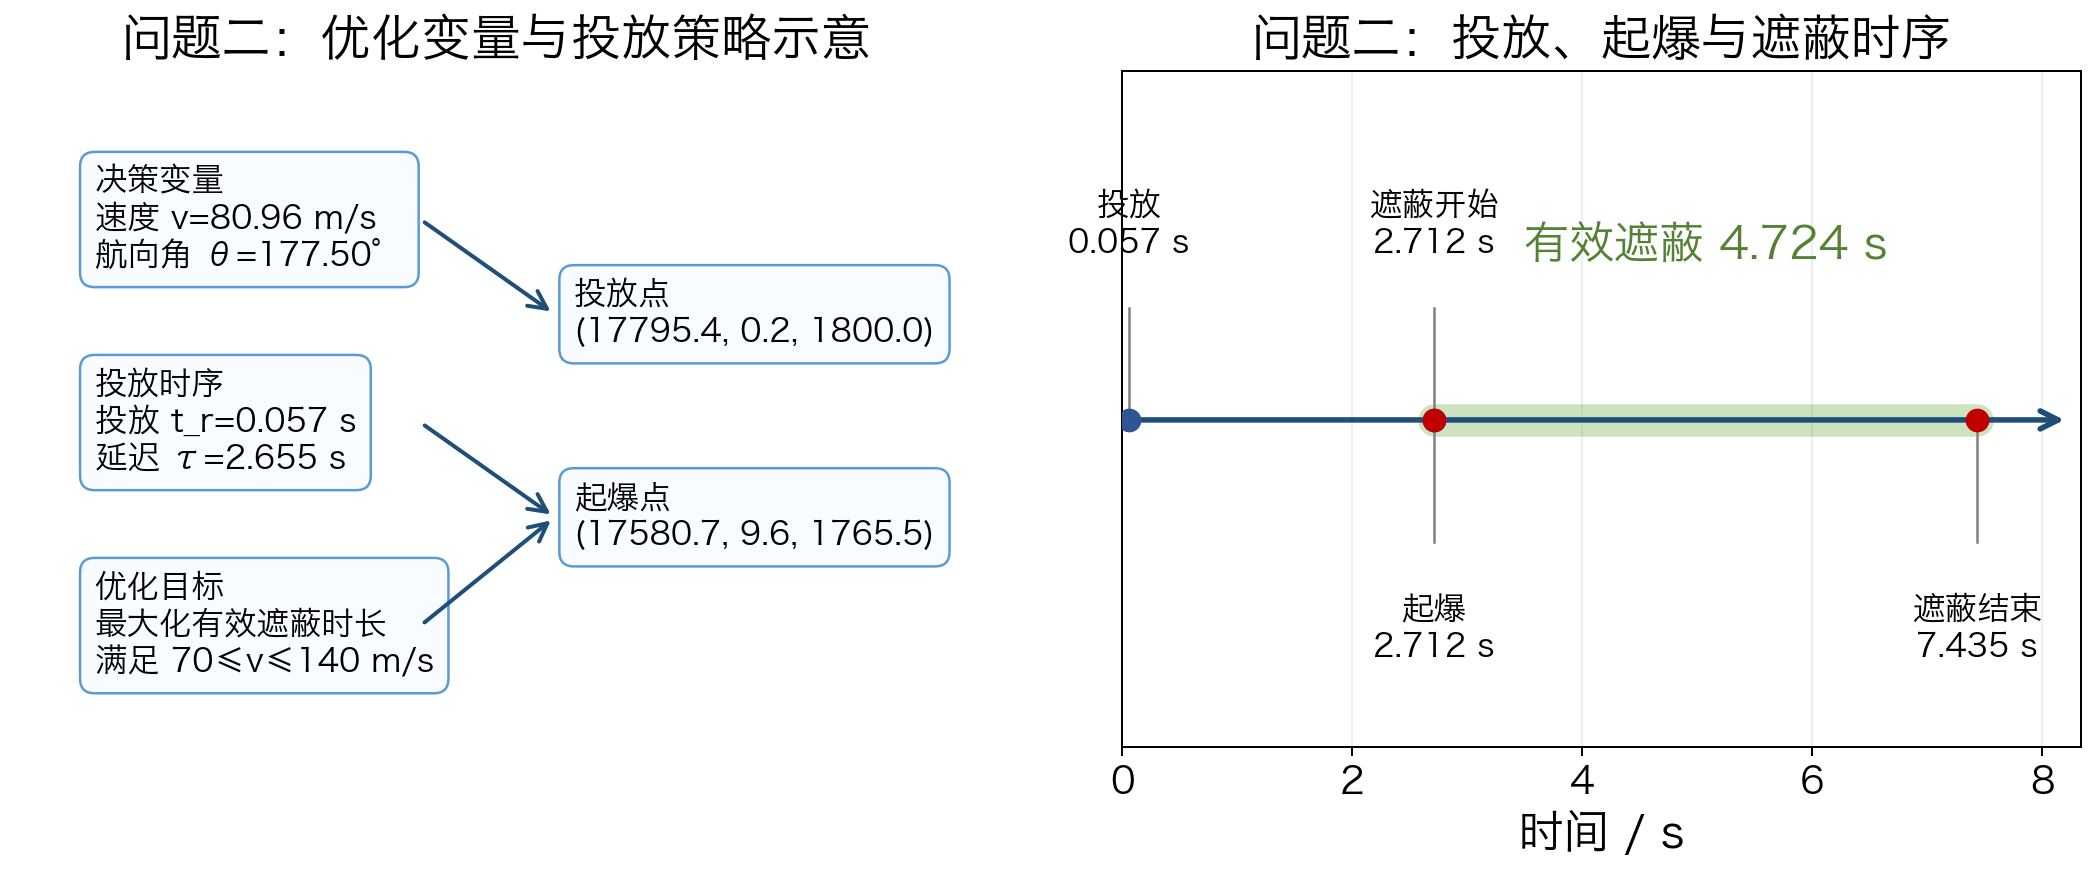
\includegraphics[width=0.94\linewidth]{../figures/fig_q2_model_schematic.png}
  \caption{问题二单机单弹策略的优化变量和投放时序示意。该图说明速度、航向、投放时刻和引信延迟如何决定投放点、起爆点和有效遮蔽区间。}
  \label{fig:q2-model-schematic}
\end{figure}

搜索得到的推荐策略见 \verb|tab_q2_strategy.csv|：FY1 速度为 \(80.963727\,\mathrm{m/s}\)，航向角为 \(3.097899251\,\mathrm{rad}\)，即从 \(x\) 轴正方向计约 \(177.496552^\circ\)。投放时刻为 \(0.056749\,\mathrm{s}\)，引信延迟为 \(2.654856\,\mathrm{s}\)，起爆时刻为 \(2.711605\,\mathrm{s}\)。对应投放点为 \((17795.409735,0.200692,1800)\)，起爆点为 \((17580.667875,9.589470,1765.463534)\)。

由 \verb|tab_q2_intervals.csv| 可知，该策略的有效遮蔽区间为 \(2.711605\sim 7.435498\,\mathrm{s}\)，有效遮蔽时长为 \(4.723893\,\mathrm{s}\)。相较问题一给定方案的 \(1.405510\,\mathrm{s}\)，该策略在示例判据下显著延长了遮蔽时间。距离曲线和侧视几何关系见图 \ref{fig:q2-distance-geometry}。

\begin{figure}[htbp]
  \centering
  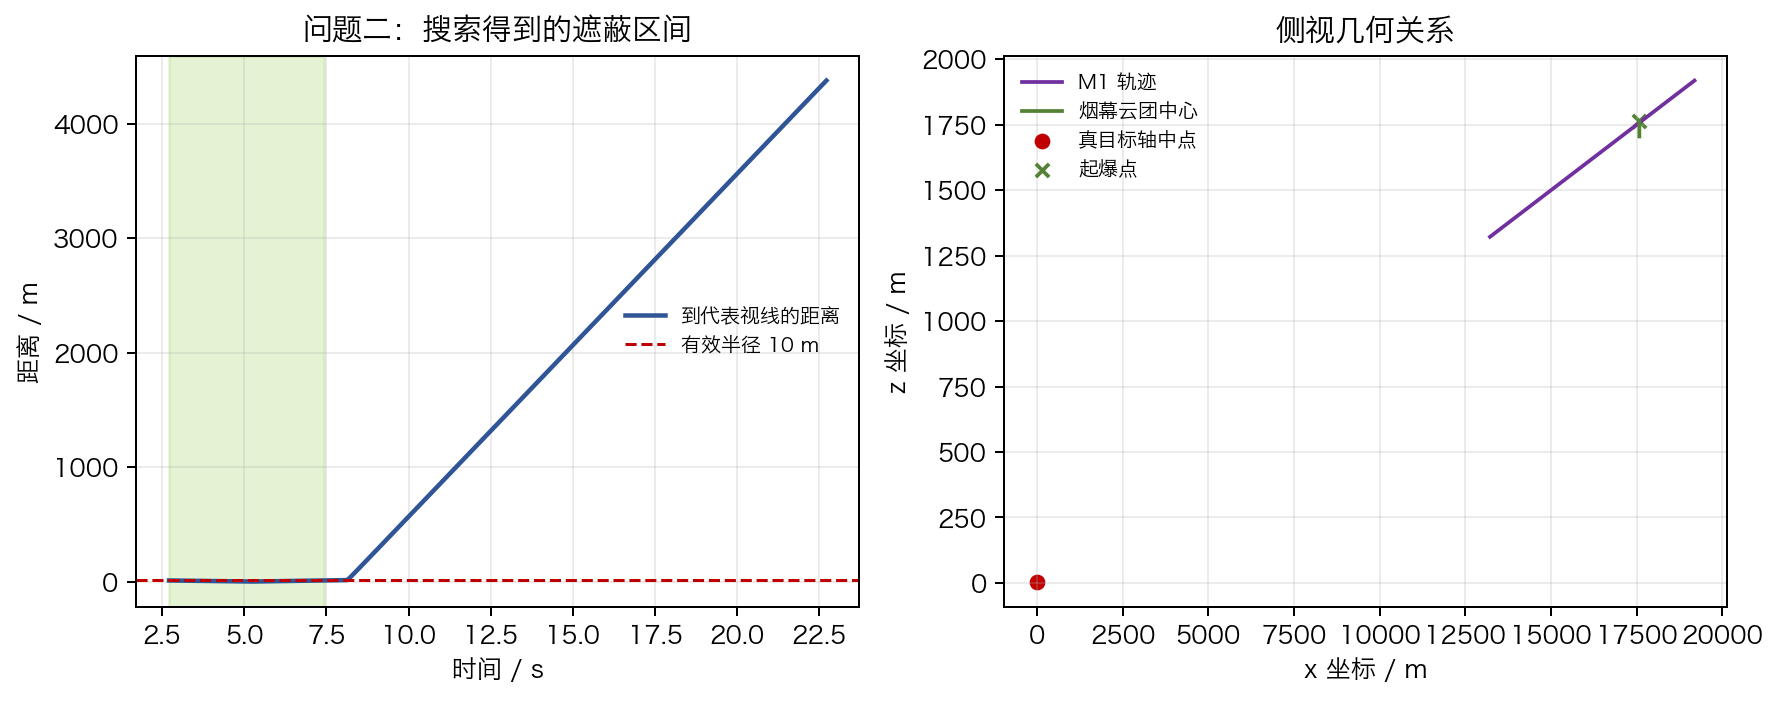
\includegraphics[width=0.92\linewidth]{../figures/fig_q2_optimized_distance_geometry.png}
  \caption{问题二推荐策略下烟幕云团到代表视线线段的距离与侧视几何示意。绿色区间表示距离不超过有效半径的时间段。}
  \label{fig:q2-distance-geometry}
\end{figure}

需要说明的是，本文示例使用确定性粗到细搜索得到 best-found 方案，尚未证明全局最优；同时，遮蔽判据仍是真目标轴中点视线判据。正式论文若采用完整圆柱目标遮蔽判据，需要进一步检查圆柱目标边界点的可见性，并重新登记结果。
